\documentclass[a4paper,12pt]{article} % добавить leqno в [] для нумерации слева
\usepackage[a4paper,top=1.3cm,bottom=2cm,left=1.5cm,right=1.5cm,marginparwidth=0.75cm]{geometry}
%%% Работа с русским языком
\usepackage{cmap}					% поиск в PDF
\usepackage{mathtext} 				% русские буквы в фомулах
\usepackage[T2A]{fontenc}			% кодировка
\usepackage[utf8]{inputenc}			% кодировка исходного текста
\usepackage[english,russian]{babel}	% локализация и переносы

\usepackage{graphicx}

\usepackage{wrapfig}
\usepackage{tabularx}

\usepackage{hyperref}
\usepackage[rgb]{xcolor}
\hypersetup{
colorlinks=true,urlcolor=blue
}
\usepackage{multirow}
\usepackage{hhline}


%%% Дополнительная работа с математикой
\usepackage{amsmath,amsfonts,amssymb,amsthm,mathtools} % AMS
\usepackage{icomma} % "Умная" запятая: $0,2$ --- число, $0, 2$ --- перечисление

%% Номера формул
\mathtoolsset{showonlyrefs=true} % Показывать номера только у тех формул, на которые есть \eqref{} в тексте.

%% Шрифты
\usepackage{euscript}	 % Шрифт Евклид
\usepackage{mathrsfs} % Красивый матшрифт

%% Свои команды
\DeclareMathOperator{\sgn}{\mathop{sgn}}

%% Перенос знаков в формулах (по Львовскому)
\newcommand*{\hm}[1]{#1\nobreak\discretionary{}
{\hbox{$\mathsurround=0pt #1$}}{}}

\begin{document}
	
	\begin{titlepage}
	\begin{center}
		{\large МОСКОВСКИЙ ФИЗИКО-ТЕХНИЧЕСКИЙ ИНСТИТУТ (НАЦИОНАЛЬНЫЙ ИССЛЕДОВАТЕЛЬСКИЙ УНИВЕРСИТЕТ)}
	\end{center}
	\begin{center}
		{\large Физтех-школа электроники, фотоники и молекулярной физики}
	\end{center}
	
	
	\vspace{4.5cm}
	{\huge
		\begin{center}
			{Лабораторная работа 6.10.4}\\
			Ядерный магнитный резонанс
		\end{center}
	}
	\vspace{2cm}
	\begin{flushright}
		{\LARGE Салтыкова Дарья \\
			\vspace{0.5cm}
			Б04-105}
	\end{flushright}
	\vspace{8cm}
	\begin{center}
		Долгопрудный 2024
	\end{center}
\end{titlepage}

\noindent \textbf{Цель работы:} вычислить магнитные моменты протона, дейтрона и ядра фтора
на основе измерения их g-факторов методом ядерного магнитного резонанса (ЯМР).

\section{Основные формулы}
	\noindent Фактор Ланде:
	\begin{equation*}
		\label{eq:g}
		\tag{$\star$}
		g_\text{я} = \frac{hf_0}{\mu_\text{я}B_0}.
	\end{equation*}
	Магнитный момент ядра:
	\begin{equation*}
		\label{eq:mu}
		\tag{$\star\star$}
		\mu = g_\text{я}\mu_\text{я}I.
	\end{equation*}
	Ядерный магнетон:
	\begin{equation*}
		\mu_{\text{я}} = \frac{e\hbar}{2m_pc} \approx 5,05\cdot10^{-27} \text{Дж}\cdot\text{Тл}^{-1}.
	\end{equation*}


\section{Экспериментальная установка}
\begin{figure}[h]
\begin{center}
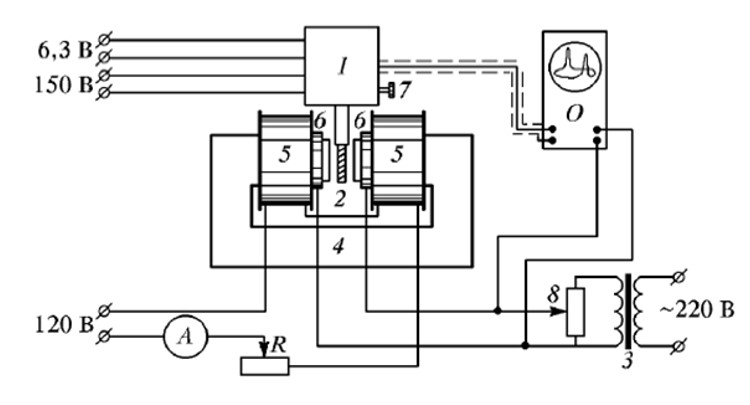
\includegraphics[width = \textwidth]{1.jpg}
\caption{Схема установки для изучения ядерного магнитного резонанса}
\end{center}
\end{figure}
В магнитном поле ядерные уровни расщепляются и под действием внешнего высокочастотного поля могут происходить электромагнитные переходы между компонентами расщепившегося уровня, это явление носит резонансный характер и потому называется ядерным магнитным резонансом. Различие по энергии между этими двумя соседними компонентами определяется формулой
\[\Delta E = g_{\text{я}}\mu_{\text{я}}B_0\]
\[f_0 = \frac{\Delta E }{h} = \frac{g_{\text{я}}\mu_{\text{я}}B_0}{h}\]

Схема экспериментальной установки представлена на рис. 1. Детектирование сигнала ЯМР осуществляется с помощью промышленного прибора. Модуляция магнитного поля осуществляется с помощью небольшой катушки, частота модуляции $\approx 50$ Гц. В зазоре электромагнита устанавливается холловский измеритель магнитного поля, а измерения ЯМР проводятся на резине (измеряется ЯМР на протонах), тефлоне (в состав входит фтор) и тяжелой воде.


\section{Результаты измерений}

Результаты измерений резонансной частоты и вычислений g-факторов и магнитных моментов представлены в таблице 1, а полученные осциллограммы на рис. 2.

\begin{figure}[h!]
\begin{minipage}[h!]{0.45\linewidth}
\center{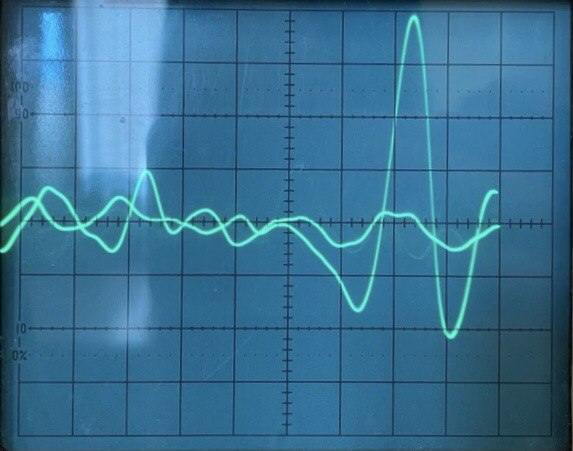
\includegraphics[width=1\linewidth]{вода.jpg}} Вода (ЯМР на протонах) \\
\end{minipage}
\hfill
\begin{minipage}[h!]{0.45\linewidth}
\center{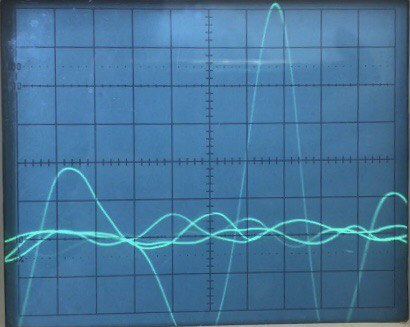
\includegraphics[width=1\linewidth]{резина.jpg}} \\ Резина (ЯМР на протонах)
\end{minipage}
\vfill
\begin{minipage}[h!]{0.45\linewidth}
\center{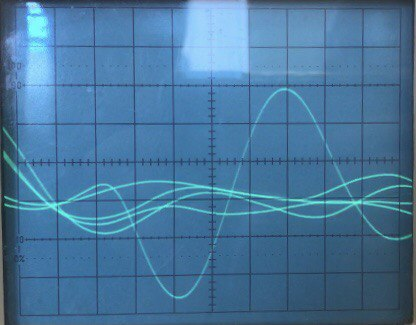
\includegraphics[width=1\linewidth]{тефлон.jpg}} Тефлон (ЯМР на ядрах фтора) \\
\end{minipage}
\hfill
\begin{minipage}[h!]{0.45\linewidth}
\center{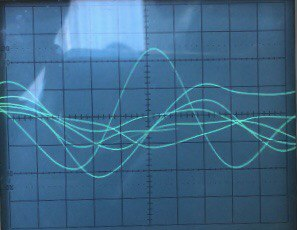
\includegraphics[width=1\linewidth]{дейтерий.jpg}} Дейтерий (ЯМР на дейтронах) \\
\end{minipage}
\caption{Осциллограммы}
\label{graphs}
\end{figure}

\begin{table}[h!]
\begin{tabular}{|c|c|c|c|c|c|c|}
\hline
Образец  & $f_0$, МГц & $B_0$, мТл & $g_{\text{я}}$ & I   & $\mu$, ед. $\mu_{\text{я}}$ & $\mu_{\text{табл}}$, ед. $\mu_{\text{я}}$ \\ \hline
Вода     & 9,913      & 229        & 5,687          & 1/2 & 2,843                       & 2,79                                      \\ \hline
Резина   & 9,816      & 231        & 5,596          & 1/2 & 2,798                       & 2,79                                      \\ \hline
Тефлон   & 9,200      & 246        & 4,917          & 1/2 & 2,459                       & 2,62                                      \\ \hline
Дейтерий & 3,317      & 526        & 0,829          & 1   & 0,829                       & 0,857                                     \\ \hline
\end{tabular}
\caption{Результаты}
\end{table}

\section{Вывод}

В ходе работы были методом ЯМР определены g-факторы и магнитные моменты протона, дейтрона и ядра фтора. Полученные данные согласуются с табличными. Заметим, что g-факторы протона и ядра фтора близки, так как спин ядра фтора 1/2. Это объясняется тем, что у фтора уровень 2s$_{1/2}$ заполняется раньше.

\end{document}